\documentclass[
  % lualatex,
  11pt,
  a4paper
]{article}

% ------------------------------ font
\usepackage{times}

% ------------------------------ math
\usepackage{amsmath,amssymb}
\usepackage{siunitx}

% ------------------------------ author & natbib
\usepackage{authblk}
\usepackage[semicolon]{natbib}
\bibliographystyle{newapa.bst}

% ------------------------------ appendix
\usepackage[title]{appendix}

% ------------------------------ tables
\usepackage{here}
\usepackage{longtable, booktabs, array}
\usepackage{threeparttable, threeparttablex, multirow}
% \newcolumntype{d}{S[input-symbols = ()]}

% ------------------------------- figures
\usepackage{graphics, graphicx}
\makeatletter
\def\maxwidth{\ifdim\Gin@nat@width>\linewidth\linewidth\else\Gin@nat@width\fi}
\def\maxheight{\ifdim\Gin@nat@height>\textheight\textheight\else\Gin@nat@height\fi}
\makeatother
% Scale images if necessary, so that they will not overflow the page
% margins by default, and it is still possible to overwrite the defaults
% using explicit options in \includegraphics[width, height, ...]{}
\setkeys{Gin}{width=\maxwidth,height=\maxheight,keepaspectratio}

% ------------------------------ page settings
\usepackage[left=3cm,right=3cm,top=3cm,bottom=3cm]{geometry}
\usepackage{setspace}
\renewcommand{\baselinestretch}{1.5}
\providecommand{\tightlist}{%
  \setlength{\itemsep}{0pt}\setlength{\parskip}{0pt}}

% ------------------------------ hyperlink
\usepackage{hyperref}

% ------------------------------ other packages
\usepackage{booktabs}
\usepackage{longtable}
\usepackage{array}
\usepackage{multirow}
\usepackage{wrapfig}
\usepackage{float}
\usepackage{colortbl}
\usepackage{pdflscape}
\usepackage{tabu}
\usepackage{threeparttable}
\usepackage{threeparttablex}
\usepackage[normalem]{ulem}
\usepackage{makecell}
\usepackage{xcolor}
\usepackage{siunitx}

  \newcolumntype{d}{S[
    input-open-uncertainty=,
    input-close-uncertainty=,
    parse-numbers = false,
    table-align-text-pre=false,
    table-align-text-post=false
  ]}
  

% ------------------------------ paper information
\title{Adding Nudge-based Reminders to Financial Incentives for Promoting Antibody Testing and Vaccination to Mitigate the Spread of Rubella\thanks{This study was conducted as a part of the ``Implementation of EBPM in Japan'' project undertaken at the Research Institute of Economy, Trade and Industry (RIETI). In completing this paper, we thank the participants of the EBPM Study Group and Discussion Paper Study Group of RIETI for their insightful comments. Before conducting the randomized controlled trial on the online survey, this study was approved by the institutional review board of the Graduate School of Economics, Osaka University {[}approval number R020114{]}. Conflict of interest: none. Funding: This research was financially supported by the Ministry of Health, Labour and Welfare, Japan; the Japan Society for the Promotion of Science {[}grant number 20H05632 (F., Ohtake){]}; and the Japan Science and Technology Agency {[}grant number JPMJPR21R4 (S., Sasaki){]}.}}
\author{}
\date{}

\begin{document}
\maketitle
\begin{abstract}
We study the effects of combining financial incentives with nudges to promote antibody testing and vaccination to mitigate the spread of rubella. In FY2019, the Japanese government began providing vouchers for free antibody testing and vaccination to men aged 40--57 years. Vouchers were automatically mailed to 40--46-year-old men in FY2019. While those aged 47--57 received vouchers after FY2020, they could obtain vouchers for undertaking antibody testing and being vaccinated in FY2019 by applying. Focusing on this policy distinction, we conduct a late-FY2019 online field experiment with Japanese 40--57-year-old men. We randomly send nudge-based text message reminders recommending antibody testing and vaccination and track self-reported behavior until the end of FY2019. One nudge-based reminder with an altruistic message on fetal harm through infection from men to pregnant women significantly promotes antibody testing and vaccination among those who have already received vouchers as a financial incentive. By contrast, nudge-based reminders have no promoting effect for those who must apply for vouchers.
\vskip\baselineskip
\noindent
\textit{Keywords}: behavioral economics, health behavior, online field experiment, rubella, vaccination, antibody test, text message reminders, free vouchers
\end{abstract}



\hypertarget{intro}{%
\section{Introduction}\label{intro}}

Vaccination is an essential countermeasure against infectious diseases, including COVID-19, seasonal influenza, and rubella. Vaccination enables individuals to voluntarily acquire antibodies and immunity. They can thus prevent the onset of infectious diseases and even infection itself.

Vaccination has positive externalities and benefits for both vaccinated individuals and the surrounding community and society. For example, vaccination lowers the risk of developing an infectious disease or becoming severely ill.~It also reduces the burden on the healthcare delivery system. Vaccination with infection-preventive effects, including the rubella vaccination, reduces both the risk of infection for the vaccinated and the risk of spreading the infection. Vaccination can thus contribute to social stability during pandemics and the acquisition of herd immunity through these positive externalities.

However, economic theories suggest that vaccination rates may not reach the socially optimal level due to such positive externalities \citep{Brito1991a, Francis1997, Stiglitz2000} under which the marginal individual benefit of vaccination is lower than the marginal social benefit. This feature could discourage vaccination by those with selfish motives. Indeed, even if people are altruistic and gain utility from the social benefits of their vaccinations reducing the probability of others becoming infected, they still have an incentive to free-ride on others' vaccinations and not receive the vaccines themselves because their probability of infection is reduced by others' vaccinations. Empirical studies report that increased rates of others' vaccinations reduce the likelihood of people being vaccinated \citep{Hershey1994, Ibuka2014}.

To overcome the challenge of vaccine coverage not achieving socially optimal levels, governments have used a variety of interventions, including monetary and non-monetary interventions (nudges in behavioral economics). Among monetary interventions, many countries subsidize vaccinations, making them free, and recent studies have confirmed the effectiveness of such measures \citep{Barber2022, Brehm2022}. Nudge-based interventions include recommending a predetermined vaccination date, sending a reminder message, and changing the message content \citep{Chapman2010, Sasaki2022, Yokum2018}.\footnote{Studies examining vaccines for seasonal influenza and COVID-19 have found that messages encouraging people to take ownership for their vaccination, such as ``A vaccine dose is reserved for you,'' promotes their vaccination uptake \citep{Dai2021, Milkman2021}.}

This study explores the possibility of combining financial incentives with nudges in vaccination and antibody acquisition. Many previous studies have estimated or compared these two interventions as independent or substitutive. However, Thaler and Sunstein defined nudges as ``an aspect of choice architecture that alters people's behaviour in a predictable way without forbidding any options or significantly changing their economic incentives'' \citep[p.6]{Thaler2009}. As mentioned, ``without significantly altering economic incentives,'' nudges include devising wordings and expressions for existing financial incentives. They further explain that nudges adjust the salience of financial incentives so that the incentives have the expected effect. Nudges and financial incentives can be complementary.

Recent studies have begun to examine the combination of nudges and financial incentives in non-vaccination contexts. For example, \citet{Burtch2018} found that combining a nudge emphasizing social norms with a financial incentive improves the length and quality of online market reviews more than either intervention alone. \citet{Thorndike2016} reported similar results for healthy food choices in a hospital cafeteria. By contrast, \citet{Kullgren2014} found that combining nudges and financial incentives does not increase outdoor exercise among older adults, while \citet{Pellerano2017} reported that adding a financial incentive to a social norm nudge undermines the energy-saving effect of the nudge-based intervention alone.\footnote{Besides field experimental studies, some laboratory experimental studies have also tested the effects of the combination. \citet{Chen2021} showed that combining a financial incentive with an informational nudge induces cooperative behavior in a prisoner's dilemma game among intrinsically motivated individuals.} However, to the best of our knowledge, no study has focused on the combination of financial incentives and nudges in the context of vaccination.

As previously stated, many previous studies have separately estimated the effects of financial incentives \citep{Banerjee2010, Barber2022, Barham2009, Brehm2022} and nudges \citep{Dai2021, Chapman2010, Milkman2021, Sasaki2022} as standalone measures. Although some have focused on both, they have compared the effects of the two interventions and regarded the two as substitutive. For example, \citet{Bronchetti2015} conducted a randomized controlled trial (RCT ) with college students in Pennsylvania and found that a financial incentive increases their seasonal influenza vaccination rate, while a peer-related nudge increases vaccine information exposure but not vaccination rates. \citet{Campos-Mercade2021a} reported that a €20 financial incentive increases vaccination rates by 4 percentage points (pp) in a Swedish field experiment and emphasized that some nudge-based interventions have little promoting effect.

Hence, we add new insights to the literature on the combination of financial incentives and nudges by focusing on Japan's policy on rubella antibody testing and vaccination and conducting a nationwide online field experiment. We estimate the effect of providing nudge-based messages in two situations: (i) people can easily obtain financial incentives and (ii) they incur additional transaction costs to obtain financial incentives. In the former situation, financial incentives and nudges are more closely combined.

In Japan, men born between April 2, 1962 and April 1, 1979 (aged 40--57 years as of 2019) have historically been excluded from routine rubella immunization (see Section \ref{background} for the details). Consequently, men in this age group have lower antibody prevalence than their female counterparts. Therefore, Japan has yet to achieve herd immunity against rubella. Unlike flu and COVID-19 vaccinations, rubella vaccine-induced immunity is long-lasting, and people without antibodies must receive a single vaccination to achieve herd immunity against rubella. The Ministry of Health, Labour and Welfare (MHLW) initiated an additional measure for the routine rubella vaccination in FY2019 by mailing vouchers covering the costs of the rubella antibody test (approximately JPY 5,000, equal to USD 45) and vaccination (approximately JPY 10,000) to men aged 40--57 years to confirm whether they have an antibody and then encourage vaccination for those without it.\footnote{We assume USD 1 = JPY 110.}

Free vouchers were distributed by local governments to men aged 40--46 years in FY2019 and those aged 47--57 years after FY2020. Men aged 47--57 years had to apply to their local government to receive the voucher during FY2019. That is, in FY2019, men aged 40--46 years received the free vouchers as financial incentives by default, whereas men aged 47--57 years had to opt in to receive the vouchers, incurring transaction costs.

We conducted an online field experiment in February and March 2020 (at the end of FY2019) with men aged 40--57 years living across Japan, including the aforementioned two age groups. We used an RCT and sent nudge-based text message reminders to encourage the uptake of antibody testing and vaccination. We ascertained their intentions to receive the test and vaccine, and their self-reported behaviors to receive them in a follow-up survey.

By focusing on the sample aged 40--46 years, we can capture the effect of providing additional text message reminders in the situation in which they already obtained the vouchers as financial incentives. Meanwhile, by using the sample aged 47--57 years, we can capture the effects of providing text message reminders in the situation in which they must incur transaction costs and opt in to obtain financial incentives. In other words , this study focuses on the combination of nudges and the costs of acquiring financial incentives. The approach of reducing these costs by delivering vouchers to the target population is observed in a variety of policy issues \citep[e.g.,][]{Ahmed2011, Kacker2022}. Therefore, exploring this realistic combination of financial incentives and nudges is important from a policy perspective.

In our experiment, we randomly offer either a control text message reminder with no nudge or one of six nudge-based text message reminders to both groups. The main finding is that a reminder with an altruistic message that emphasizes the negative impact on newborns caused by infection from the men to pregnant women is effective in promoting antibody testing and increasing the vaccination rate only in the sample that obtains the financial incentive by default.

This study contributes to the literature exploring the conditions under which nudges work effectively. Evidence for the effectiveness of nudges has recently been mixed. According to the meta-analysis by \citet{DellaVigna2022a}, nudges are infrequently used in reality and their effectiveness depends on various conditions, including topics and channels. This study demonstrates that nudges can be effective when given to a group that has already obtained financial incentives. This result is also consistent with the original definition of the two being complementary.

This research also contributes to the literature by supporting the global effort to acquire herd immunity against rubella. According to the World Health Organization, 101 of 194 countries have not yet eliminated rubella \citep{Zimmerman2022}. Specifically, in the Eastern Mediterranean, South-East Asia, and Western Pacific regions, the proportion of countries that have not yet achieved herd immunity is high. By contrast, Japan is extremely close to achieving herd immunity. As cross-border traffic increases after the end of the COVID-19 pandemic, achieving herd immunity against rubella will become increasingly important for these lagging countries.

The rest of this paper is structured as follows. Section \ref{background} provides an overview of rubella in Japan. Section \ref{experiment} describes the experimental design and Section \ref{results} presents the results. Finally, Section \ref{conclusion} discuss the results and concludes.

\hypertarget{background}{%
\section{Background of Rubella Vaccination in Japan}\label{background}}

Rubella is a highly contagious disease spread through droplet transmission. The most common symptoms are fever and rashes, but the disease is rarely severe.\footnote{According to the National Institute of Infectious Diseases (NIID), the subclinical transmission of rubella (the state in which a person is infected but has no symptoms) occurs in approximately 15--30\% of cases. Fever is observed in approximately 50\% of patients. Adults may also experience transient arthritis (5--30\%). Rarely, complications such as thrombocytopenic purpura (\(0.02\)--\(0.03\)\%) and acute encephalitis (\(0.01\)--\(0.03\)\%) may require hospitalization (\url{https://www.niid.go.jp/niid/ja/kansennohanashi/430-rubella-intro.html}. Japanese. Accessed September 22, 2023).} The most serious problem is that women infected with rubella during early pregnancy may have children with congenital rubella syndrome (CRS), which includes eye and ear defects. Because the spread of rubella tends to increase the CRS incidence, the Japanese government has designated rubella as a disease requiring immunization. According to \citet{Kinoshita2016}, Japan can obtain herd immunity against rubella if the antibody prevalence exceeds 90\% in all generations.\footnote{According to \citet{Plans-Rubio2012}, an antibody prevalence of 83--95\% achieves herd immunity against rubella. \citet{Nishiura2015} found that the antibody prevalence for herd immunity is 83.6\%.}

\begin{figure}[t]
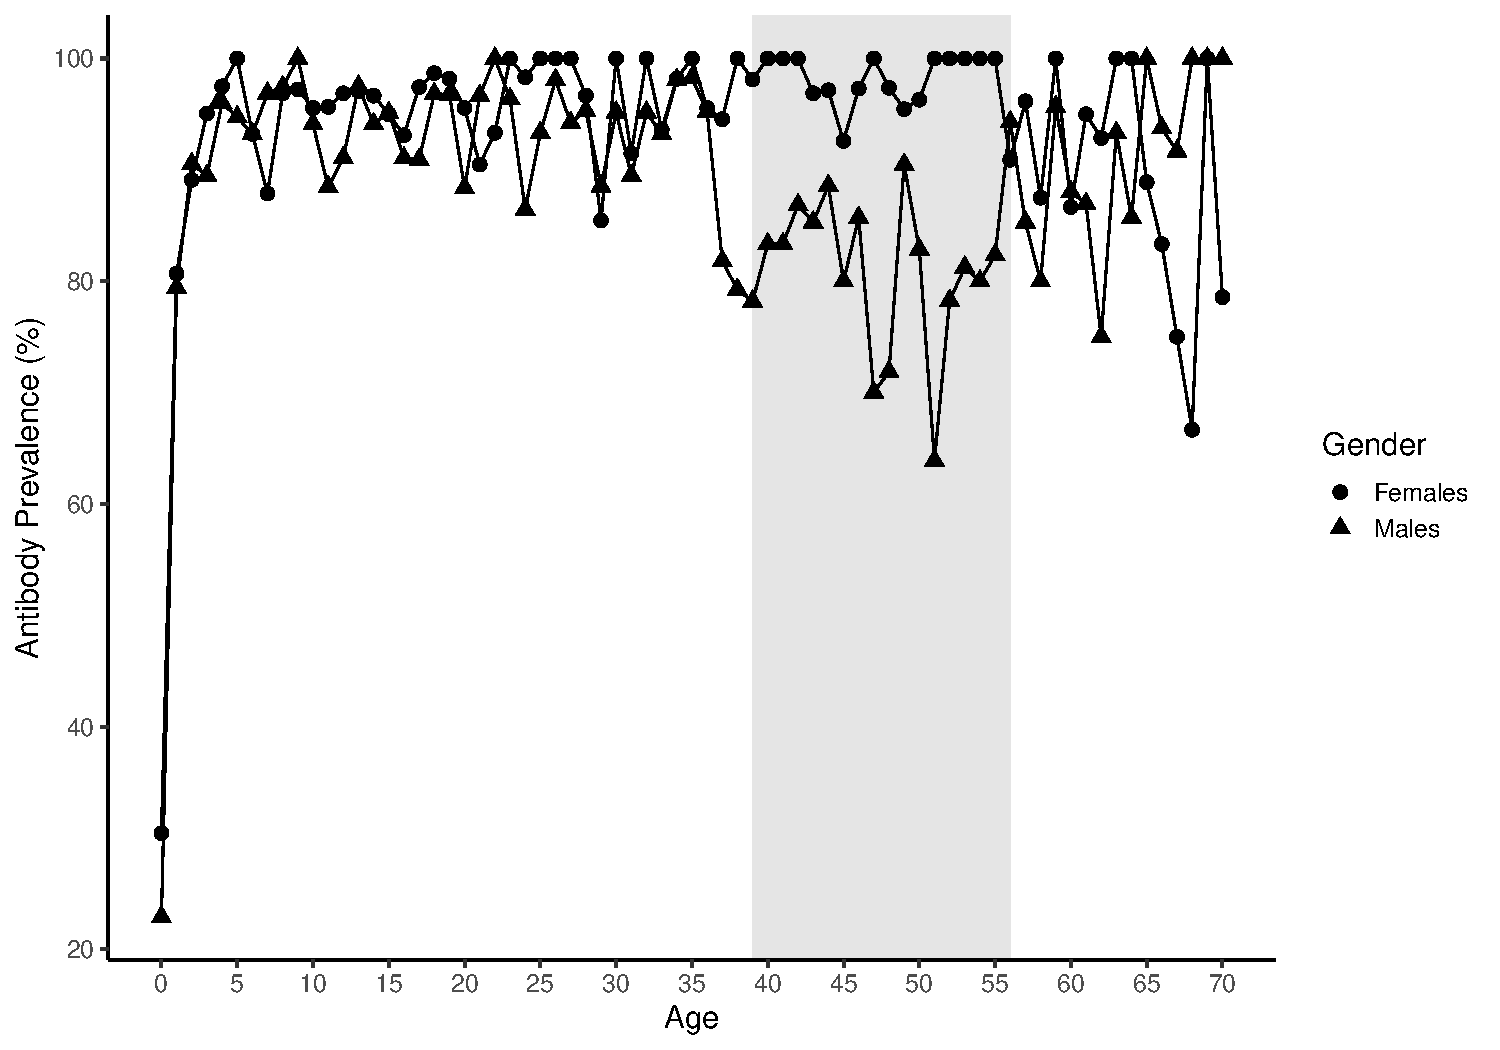
\includegraphics{Main-Document-LaTeX_files/figure-latex/antibody-1} \caption{Percentage of Rubella Antibody Prevalence by Age and Gender. Data: 2018 National Epidemiological Surveillance of Vaccine-Preventable Diseases, NIID}\label{fig:antibody}
\end{figure}

However, owing to low antibody prevalence among men in their 40s and 50s, Japan has not achieved herd immunity to rubella. Figure \ref{fig:antibody} shows that the antibody prevalence among men aged 39--56 years (as of 2018) is approximately 81.5\%, which is lower than that of women of the same generation (about 97.9\%) and other generations because they have not received their routine rubella vaccination and have not had less opportunity to infect naturally.\footnote{The prevalence rates of antibodies in men and women aged 57 and older are 91.1\% and 89.3\%, respectively. Despite not having received routine vaccination, men and women aged 57 and older grew up during a time when rubella was common and people are likely to have antibodies from natural infection. The antibody prevalence of men and women aged 38 years and younger is 91.3\% and 94.0\%, respectively. They have had at least one dose of the rubella vaccine administered as part of routine immunization.} Thus, the influx of viruses of Southeast Asian origin caused rubella epidemics in 2013 and 2018, mainly among men with relatively low antibody prevalence \citep{NIID2019}.\footnote{In the 2018 epidemic, the U.S. Centers for Disease Control and Prevention advised pregnant women not to travel to Japan (The Japan Times, October 24, 2018. \url{https://www.japantimes.co.jp/news/2018/10/24/national/science-health/u-s-cdc-warns-pregnant-women-traveling-japan-amid-rubella-outbreak/}. Accessed September 22, 2023).} As cross-border traffic is increasing, achieving herd immunity against rubella is becoming increasingly important for Japan.\footnote{If transmission to pregnant women is the most important issue, one might think that vaccinating pregnant women would be the optimal strategy. However, Japan implemented measures for pregnant women in advance of the 2019 vaccination campaign, as they were already receiving at least one vaccination. In addition, since 2014, pregnant women and women who want to become pregnant as well as their partners have been offered free antibody testing. However, during the 2013 and 2018 epidemics, some infants were affected by CRS. Therefore, to eradicate CRS, interventions for pregnant women alone are insufficient; interventions to achieve hard immunity are needed.}

To achieve herd immunity, Japan must raise the antibody prevalence among men in their 40s and 50s from 80\% to 90\%. To achieve this goal, the MHLW provided the rubella vaccination as an additional free routine immunization for men aged 40--57 years (as of 2019) between April 2019 and March 2022.\footnote{More precisely, eligible men were born between April 2, 1962 and April 1, 1979.} Eligible men had to first receive antibody testing. Men who returned a negative test were then vaccinated.

Under the Immunization Act, eligible men receive free antibody testing and vaccinations. The MHLW requested local governments to send free vouchers for a rubella antibody test and vaccine to eligible men over a three-year period. This setting provides a natural experimental setting under which we can divide eligible men into the following two age groups depending on whether they automatically received the voucher in FY2019:

\begin{enumerate}
\def\labelenumi{\arabic{enumi}.}
\tightlist
\item
  40--46 years old: automatically received the free voucher in FY2019;
\item
  47--57 years old: automatically received the free voucher after FY2020 but had to apply to obtain it in FY2019.
\end{enumerate}

Thus, the transaction costs for the financial incentives in FY2019 differ between the age groups. In particular, 40--46-year-old men incur no transaction costs because they obtained the financial incentives by default in the form of free vouchers in FY2019 (\emph{default incentive} group). However, 47--57-year-old men have high transaction costs (e.g., travel costs to a city hall) because they had to contact their local government to obtain the free vouchers in FY2019 (\emph{opt-in incentive} group).\footnote{One local government posted the application forms on its website. To obtain a vaccination voucher, eligible men had to download and complete the forms, and either mail them to the local government or visit the city hall in person. The cost of obtaining the documents and traveling to the city hall thus seems to be significant.}

However, although men aged 40--46 years automatically received the financial incentives, the actual uptake of antibody testing with vouchers remained as low as 18\% as of January 2020.\footnote{More than half of eligible men are 40--46 years old (\(6.46\) million). They received the free vouchers from April 2019 to March 2020. According to interviews conducted by the MHLW, approximately 96\% of local governments planned to send the vouchers by October 2019. The cumulative number of antibody tests using vouchers by January 2019 was 1.17 million. We calculate the actual uptake of antibody testing by dividing the cumulative number of antibody tests using vouchers to January 2019 (\(1.17\) million) by the population of 40--46-year-old men (\(6.46\) million).}

\hypertarget{experiment}{%
\section{Nationwide Online Survey Experiment}\label{experiment}}

\hypertarget{intervention}{%
\subsection{Non-Monetary Interventions: Text Message Reminders}\label{intervention}}

When the financial incentives offered are adequate, as in the presented case, non-monetary interventions should be considered to increase antibody testing. In this study, we developed seven nudge-based text message reminders for those who remained untested and unvaccinated (see Table \ref{tab:message-list}).

\begin{table}

\caption{\label{tab:message-list}List of the Text Message Reminders}
\centering
\fontsize{9}{11}\selectfont
\begin{tabular}[t]{l>{\raggedright\arraybackslash}p{20em}cccccc}
\toprule
\multicolumn{3}{c}{ } & \multicolumn{4}{c}{Age (as of April 2019)} & \multicolumn{1}{c}{ } \\
\cmidrule(l{3pt}r{3pt}){4-7}
Message & Content &   & 39 & 40--46 & 47--56 & 57--59 & All\\
\midrule
MHLW (Control) & Dear men born between 1962 and 1979. Undertake rubella antibody testing and be vaccinated to protect yourself and the future generation! & N & 20 & 210 & 321 & 49 & 600\\
\addlinespace
MHLW (Age) & Dear men in their 40s and 50s (all men born between 1962 and 1979). Undertake rubella antibody testing and be vaccinated to protect yourself and the future generation! & N & 23 & 205 & 309 & 63 & 600\\
\addlinespace
Altruistic & Dear men in their 40s and 50s (all men born between 1962 and 1979). If you get a pregnant woman infected with rubella, she may give birth to a child with a serious disability. Undertake rubella antibody testing and be vaccinated! & N & 24 & 214 & 296 & 66 & 600\\
\addlinespace
Selfish & Dear men in their 40s and 50s (all men born between 1962 and 1979). Rubella infection in adult men may have serious complications such as encephalitis and thrombocytopenic purpura. Undertake rubella antibody testing and be vaccinated! & N & 16 & 225 & 302 & 57 & 600\\
\addlinespace
Social Comparison & Dear men in their 40s and 50s (all men born between 1962 and 1979). Compared with other generations, more than twice as many people in your generation can contract rubella because one in five of you does not have rubella antibodies. Undertake rubella antibody testing and be vaccinated! & N & 18 & 204 & 321 & 57 & 600\\
\addlinespace
Deadline & Dear men in their 40s and 50s (all men born between 1962 and 1979). The voucher for a free rubella antibody test and vaccine is valid until March 31, 2020 . Undertake rubella antibody testing and be vaccinated! & N & 18 & 216 & 299 & 67 & 600\\
\addlinespace
Convenient & Dear men in their 40s and 50s (all men born between 1962 and 1979). You can use your voucher for a rubella antibody test at a growing number of workplaces and government agencies, in addition to your usual health examinations. Undertake rubella antibody testing and be vaccinated! & N & 19 & 213 & 307 & 61 & 600\\
\bottomrule
\end{tabular}
\end{table}

Using the \emph{MHLW (Control)} message, the MHLW promotes antibody testing and vaccination against rubella on its website (business-as-usual control). We developed six additional text message reminders based on the MHLW (Control) message to explore what elements to use and how to emphasize them. Recent behavioral science research has increasingly investigated the efficacy of multiple candidate messages \citep[e.g.,][\citet{Milkman2021}]{Dai2021}, similar to this study.

The six additional text message reminders altered the MHLW (Control) message in two ways: (1) using a simple age expression (first sentence) and (2) adapting the message content (subsequent sentences). In addition to the precise target age for the additional rubella measures, the \emph{MHLW (Age)} message included the simple phrase ``men in their 40s and 50s,'''' which helped the reader understand if they are eligible for vaccination and pay attention to the message. The MHLW (Age) message only changed the age expression; the message's content was identical to the control.

The \emph{Altruistic} message described how one's infection can harm others, particularly pregnant women and their children. As previously stated, vaccination has positive externalities. In the case of rubella, having antibodies through vaccination prevents infection in pregnant women, thus protecting their children. The Altruistic message is the inverse of this positive externality, emphasizing the negative externality of not being vaccinated. This message was intended to help altruistic readers imagine the negative externalities caused by the infection and change their behavior.\footnote{We defined an altruistic person as someone who considers social benefits, including externalities.}

The \emph{Selfish} and \emph{Social Comparison} messages aimed to change behavior by increasing the importance of having rubella antibodies. The first message described the damage caused by the infection to the individual, making it easier for the reader to imagine it. The second message informed the reader that antibody prevalence is low and reminded them that they are susceptible to infection to help people avoid underestimating the likelihood of infection and undervaluing vaccination.

The \emph{Deadline} and \emph{Convenient} messages described the 2019 vaccination campaign. The first message emphasized that the FY2019 vouchers were valid until the end of March. This message aimed to prevent people from postponing antibody testing and vaccination due to present bias \citep{ODonoghue2001}. Meanwhile, the second message stated that some people can obtain antibody testing as part of a regular health examination and emphasized its convenience to reduce the subjective testing cost.

\hypertarget{survey}{%
\subsection{Nationwide Online Survey}\label{survey}}

Using a nationwide online survey, we then tested the extent to which those text message reminders improved the actual uptake of antibody testing and vaccination rate in the \emph{default incentive} group and the effect on those who incurred transaction costs to obtain them. In collaboration with the MHLW, we commissioned MyVoiceCome to conduct two surveys at the end of FY2019. On February 15--17, 2020, we conducted the first survey (Wave 1) of 4,200 Japanese men aged 40--59 years living across Japan. Wave 1 randomized the seven text message reminders. On March 17--25, 2020, we surveyed Wave 1 respondents again for the second survey (Wave 2). We received responses from 3,963 individuals (attrition rate = \(5.64\)\%).\footnote{The seven experimental arms had similar attrition rates. We linearly regressed an attrition dummy on the treatment group dummies. The F-test result for the joint null hypothesis was not statistically significant (F-value = \(1.434\); p-value = \(0.197\)).} Wave 2 aimed to test how the randomly assigned text message reminders in Wave 1 affected the actual uptake of antibody testing and vaccination rates. We obtained prior approval from the institutional review board of the Graduate School of Economics, Osaka University (approval number: R020114) for conducting the RCT on the online survey.

\hypertarget{wave1}{%
\subsubsection{Wave 1: Outcome Variables for Intention}\label{wave1}}

In Wave 1, we randomly sent one of the text message reminders in Table \ref{tab:message-list}. We employed stratified randomization. The survey firm divided respondents into four age groups (40--44, 45--49, 50--54, and 55--59) and equally assigned the messages within each group. The sample size for each group was 1,050, with 150 for one experimental arm within a group. Thus, the sample size for one experimental group was 600.\footnote{The ages shown in Table \ref{tab:message-list} are as of April 2019, calculated using the year and month of the respondents' birth. Men aged 40--56 years as of April 2019 are eligible for the MHLW's additional measures. Those aged 40--46 years automatically receive vouchers for the first year. We assume that those born in April have not yet reached their birthday. In addition, some men aged 39 years as of April 2019 were 40 years at the time of the survey.}

After viewing their randomly assigned message, the participants expressed their intention to undertake antibody testing and be vaccinated on a 5-point Likert scale (5 = definitely yes; 1 = absolutely no). The question on the willingness to undertake antibody testing was, ``Are you willing to take an antibody test for rubella now?'' Meanwhile, the intention to be vaccinated question asked, ``If the antibody testing reveals that you have no antibodies, are you willing to be vaccinated?'' We created a binary variable coded 1 if the participant responded 4 or 5 to each question and used it as the outcome variable for intention.

Before reading the randomly assigned message, the participants were asked about their economic preferences such as their altruism, daily health behavior, rubella knowledge, and willingness to pay (WTP) for the rubella vaccination. At the end of survey, they were asked about their socioeconomic status. We used these variables to perform regressions and balance checks as well as explore influencing mechanisms. See Table 1 in Supplementary Material C for variables used in the regression analysis and balance checks.

\hypertarget{wave2}{%
\subsubsection{Wave 2: Outcome Variables for Behavior}\label{wave2}}

In Wave 2, we investigated the actual uptake of antibody testing and vaccination rates after Wave 1. Supplementary Material A presents the questions on antibody testing and vaccination and the multiple-choice answers. We created a binary variable coded 1 if the respondent had undertaken antibody testing after Wave 1.

As stated earlier, to receive the rubella vaccination through routine immunization, eligible men must first undergo antibody testing. However, they may have been vaccinated against rubella at their own expense without having their antibodies tested. To eliminate this possibility, we created a binary variable coded 1 if the respondents had been tested and vaccinated after Wave 1, which we used as the outcome variable for vaccination.

Although self-reported behavioral measures may be subject to the experimenter demand effect and social desirability bias, the design and analysis of the current study addressed these biases in the following two ways. First, because this study is an RCT, these biases, if they exist to the same extent in each group, are not fatal to the identification of treatment effects. Second, even if these biases differ by group, our analysis directly controlled for the respondents' psychological factors potentially associated with these biases (e.g., following social norms, accepting bad behavior in anonymous conditions) and then estimated the treatment effects .

\hypertarget{results}{%
\section{Results}\label{results}}

\hypertarget{sample}{%
\subsection{Study Population}\label{sample}}

Our target population is men who did not undertake antibody testing or receive a vaccination. We thus exclude those respondents who stated in Wave 1 that they had already undertaken antibody testing or been vaccinated. In Wave 2, we again ask the respondents whether they had already undergone testing or received a vaccination by Wave 1. This is because they respondents may check vaccination history after wave 1 and their responses may be different from Wave 1. Thus, when estimating the effect on behavior, we exclude the respondents who stated in either wave that they had received antibody testing or been vaccinated before Wave 1.

\hypertarget{intention}{%
\subsection{Effect of the Text Message Reminders on Intention}\label{intention}}

The participants' observable characteristics are balanced across the experimental arms in both \emph{default incentive} and \emph{opt-in incentive} group (Table 2 and 3 in Supplementary Material C). Thus, we first report the difference-in-mean test (t-test) for each group.

\hypertarget{difference-in-mean-test}{%
\subsubsection{Difference-in-mean Test}\label{difference-in-mean-test}}

\begin{figure}[t]
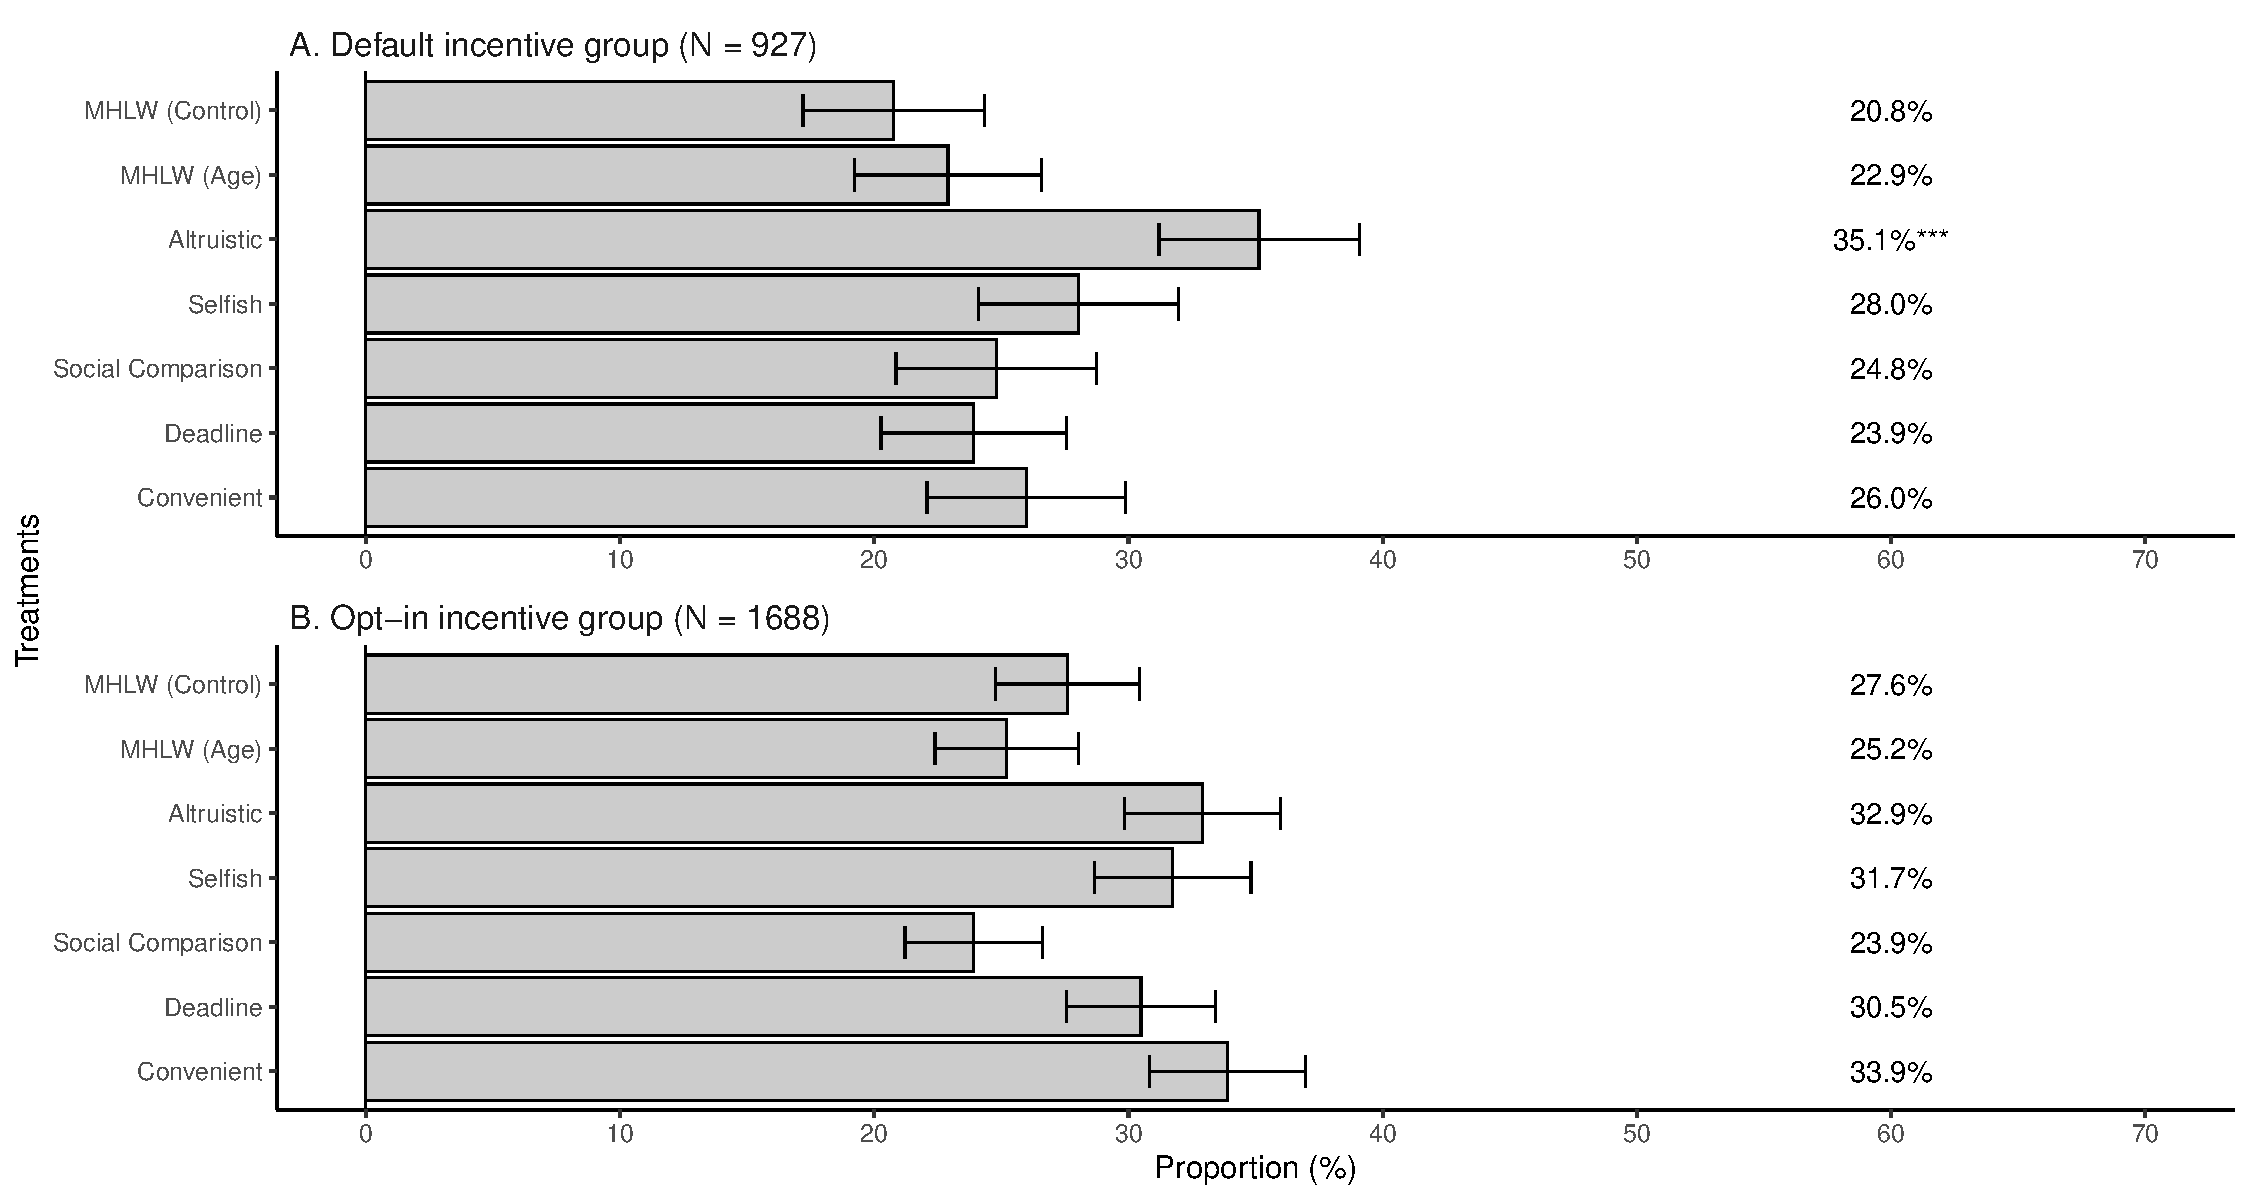
\includegraphics{Main-Document-LaTeX_files/figure-latex/ttest-int-test-1} \caption{Effect of the Text Message Reminders on the Intention to Undertake Antibody Testing. Notes: Numbers in the figure indicate the proportion of each experimental arm. Error bars indicate the standard error of the mean. Asterisks are p-values of t-tests for the difference-in-mean: * $p < 0.1$, ** $p < 0.05$, *** $p < 0.01$.}\label{fig:ttest-int-test}
\end{figure}

Figure \ref{fig:ttest-int-test} shows the intention to undertake antibody testing in each experimental arm for the \emph{default incentive} group (Panel A) and \emph{opt-in incentive} group (Panel B). In the \emph{default incentive} group, the Altruistic message increases the intention to undertake antibody testing by a statistically significant \(14.3\) pp compared with the MHLW (Control) message (\(35.1\)\% in the Altruistic message group versus \(20.8\)\% in the MHLW (Control) message group). On the contrary , in the \emph{opt-in incentive} group, the Altruistic message increases the intention to undertake antibody testing by \(5.3\) pp, which is not statistically significant (\(32.9\)\% in the Altruistic message group versus \(27.6\)\% in the MHLW (Control) message group). The effect of the Altruistic message could differ between the two groups, as the subsequent regression analysis also suggests.

\begin{figure}[t]
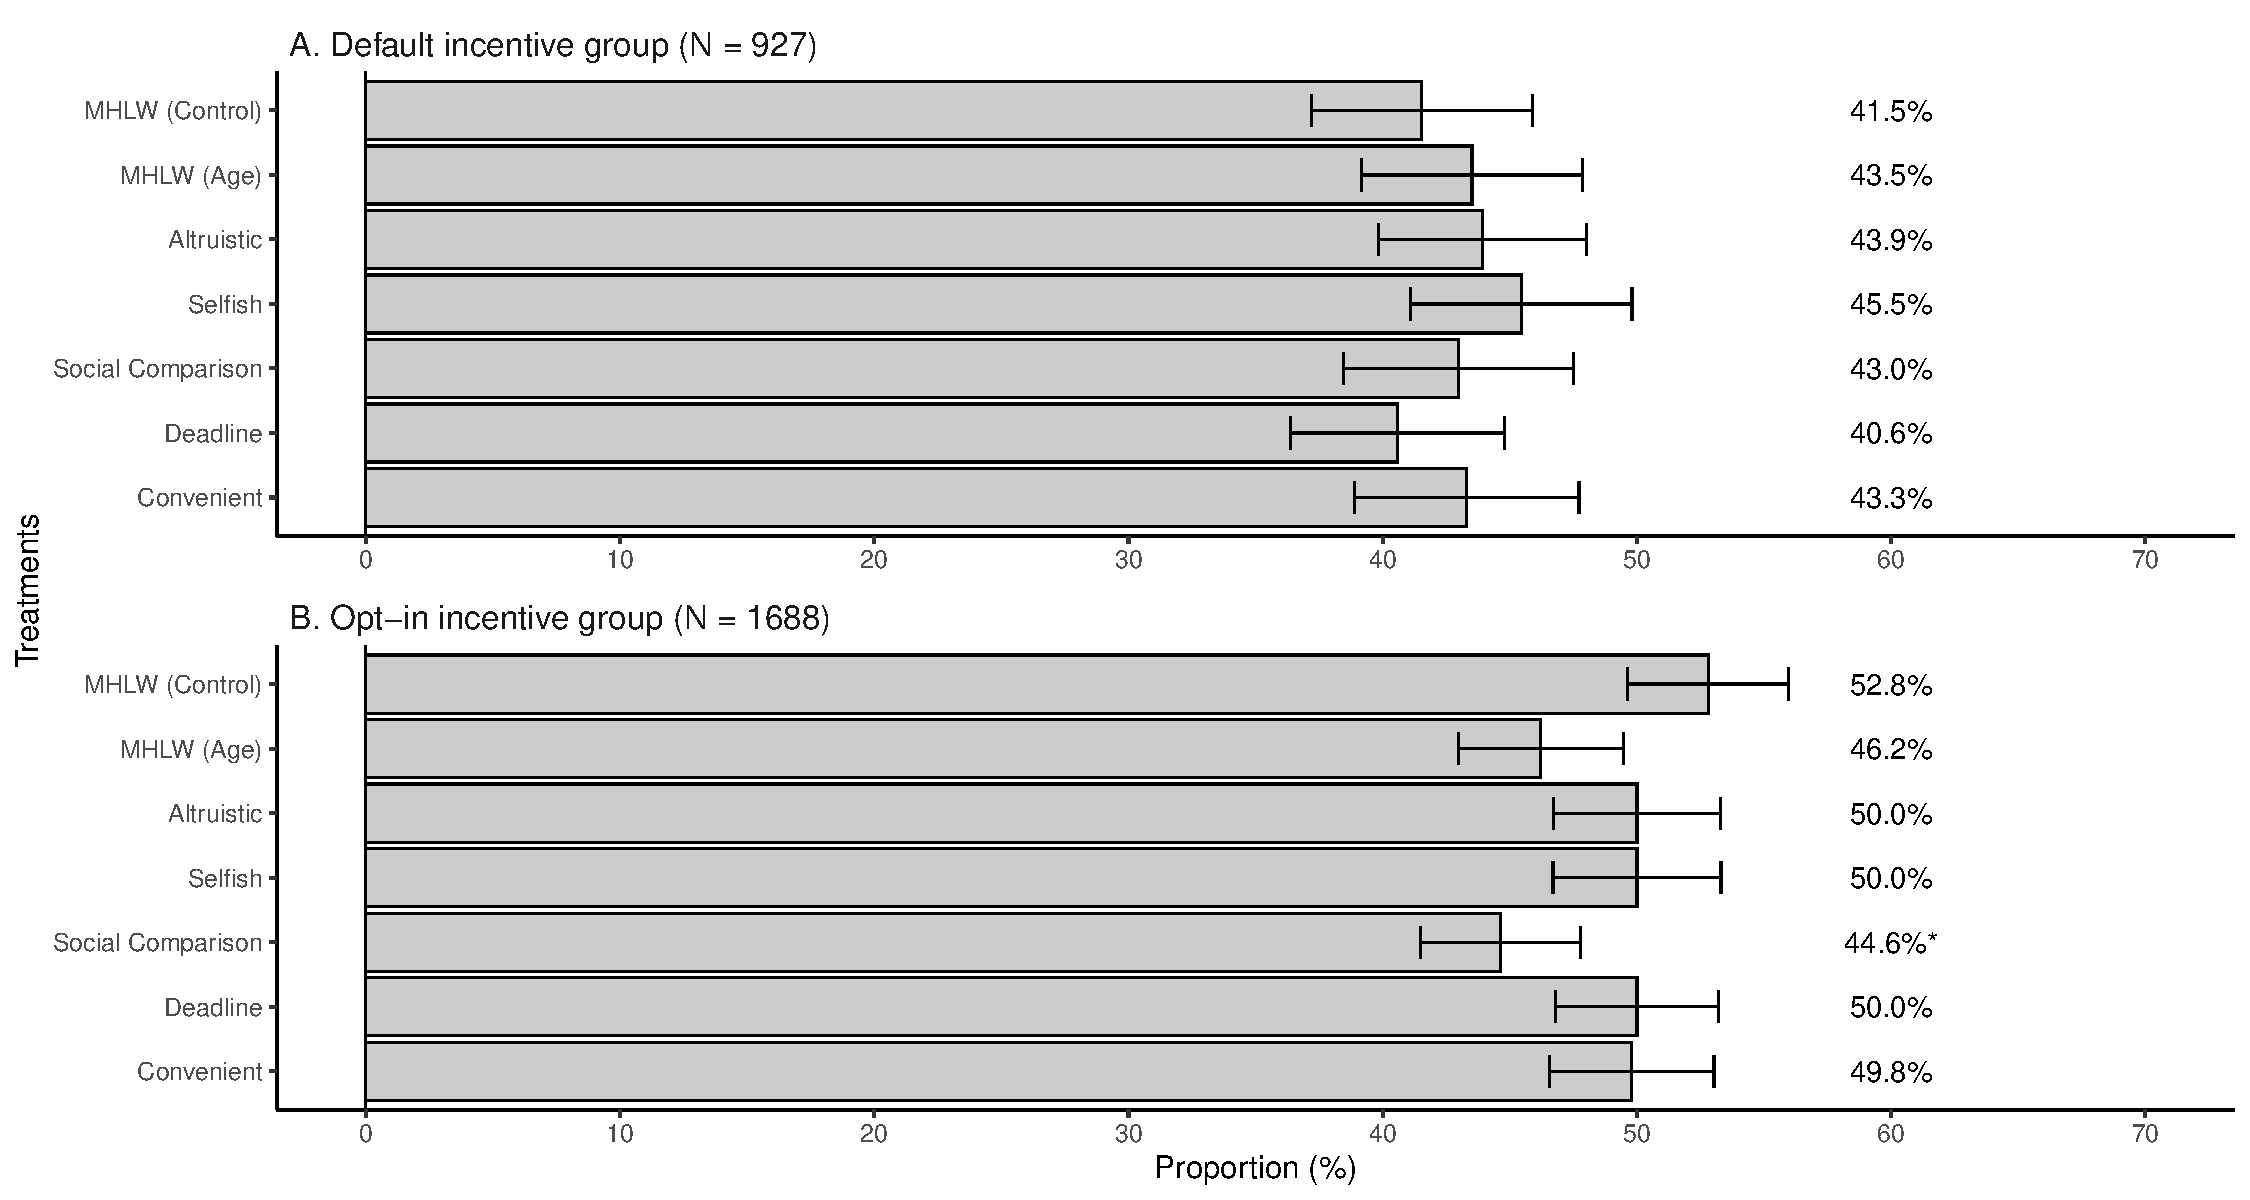
\includegraphics{Main-Document-LaTeX_files/figure-latex/ttest-int-vacc-1} \caption{Effect of the Text Message Reminders on the Intention to be Vaccinated. Notes: Numbers in the figure indicate the proportion of each experimental arm. Error bars indicate the standard error of the mean. Asterisks are p-values of t-tests for the difference-in-mean: * $p < 0.1$, ** $p < 0.05$, *** $p < 0.01$.}\label{fig:ttest-int-vacc}
\end{figure}

Figure \ref{fig:ttest-int-vacc} depicts the intention to be vaccinated for the \emph{default incentive} group (Panel A) and \emph{opt-in incentive} group (Panel B). In both incentive groups, most of the text message reminders, including the Altruistic message, do not statistically significantly increase the intention to be vaccinated compared with MHLW (Control). In the \emph{opt-in incentive} group, the Social Comparison message may lower the intention to be vaccinated compared with the MHLW (Control) message (\(44.6\)\% in the Social Comparison message group versus \(52.8\)\% in the MHLW (Control) message group).\footnote{Free-riding may explain why the Social Comparison message does not increase the intention to be vaccinated. The Social Comparison message emphasizes that ``one in five people do not have antibodies.'' Conversely, four out of five individuals have antibodies. The readers of such a message may have believed that even if they lacked rubella antibodies, the likelihood of infection would be low because 80\% of the population possesses them. When eligible men were required to undergo costly procedures to receive free vouchers, this belief may have made vaccination less beneficial.}

The intention to be vaccinated in all the experimental arms is higher than that to undertake antibody testing in both the incentive groups. This result may be explained by the stimulus of the question eliciting the intention to be vaccinated. We asked respondents to report their willingness to be vaccinated if they did not have antibodies. This condition may strongly stimulate the need for vaccination. Thus, when assessed by actual behavior, the results may differ.

\hypertarget{regression-analysis}{%
\subsubsection{Regression Analysis}\label{regression-analysis}}

Since age determines whether eligible men received the free vouchers automatically in FY2019, the different effects of the text message reminders for the two groups are influenced by the presence or absence of financial incentives as well as the differences in other factors (especially age). This motivates us to estimate the following linear probability model:
\begin{equation}
\begin{split}
Y_{ij} = &\alpha + \sum_j \beta_j \text{Message}_j + \sum_j \gamma_j (\text{Message}_j \times \text{Opt-in}_i) + \delta \text{Opt-in}_i \\
&+ \lambda X'_{ij} + \epsilon_{ij},
\end{split} \label{eq:regression}
\end{equation}
where \(\text{Message}_j\) is a treatment dummy (the reference group is MHLW (Control)), \(\text{Opt-in}_i\) is a binary variable indicating the \emph{opt-in incentive} group, and \(X\) is a set of covariates including age. Our parameters of interest are \(\beta_j\) and \(\gamma_j\). \(\beta_j\) represents the effect of the text message reminders for the \emph{default incentive} group. The linear combination of the parameters, \(\beta_j + \gamma_j\), is the effect of the text message reminders for the \emph{opt-in incentive} group. The parameter \(\gamma_j\) shows the difference in the effect of the text message reminders between the two groups.

\begin{table}

\caption{\label{tab:reg-int}Regressions of Intention}
\centering
\fontsize{9}{11}\selectfont
\begin{threeparttable}
\begin{tabular}[t]{lcccc}
\toprule
\multicolumn{1}{c}{ } & \multicolumn{2}{c}{Testing} & \multicolumn{2}{c}{Vaccination} \\
\cmidrule(l{3pt}r{3pt}){2-3} \cmidrule(l{3pt}r{3pt}){4-5}
  & (1) & (2) & (3) & (4)\\
\midrule
MHLW (Age) & \num{0.021} & \num{0.038} & \num{0.020} & \num{0.049}\\
 & (\num{0.051}) & (\num{0.048}) & (\num{0.061}) & (\num{0.058})\\
Altruistic & \num{0.144}*** & \num{0.161}*** & \num{0.024} & \num{0.048}\\
 & (\num{0.053}) & (\num{0.050}) & (\num{0.060}) & (\num{0.057})\\
Selfish & \num{0.073} & \num{0.115}** & \num{0.039} & \num{0.091}\\
 & (\num{0.053}) & (\num{0.050}) & (\num{0.061}) & (\num{0.057})\\
Social Comparison & \num{0.040} & \num{0.075} & \num{0.014} & \num{0.052}\\
 & (\num{0.053}) & (\num{0.050}) & (\num{0.063}) & (\num{0.058})\\
Deadline & \num{0.031} & \num{0.041} & \num{-0.010} & \num{0.010}\\
 & (\num{0.051}) & (\num{0.048}) & (\num{0.060}) & (\num{0.057})\\
Convenient & \num{0.052} & \num{0.060} & \num{0.018} & \num{0.034}\\
 & (\num{0.053}) & (\num{0.050}) & (\num{0.062}) & (\num{0.058})\\
Opt-in & \num{0.068} & \num{0.083}* & \num{0.113}** & \num{0.081}\\
 & (\num{0.046}) & (\num{0.050}) & (\num{0.054}) & (\num{0.059})\\
MHLW (Age) $\times$ Opt-in & \num{-0.045} & \num{-0.078} & \num{-0.086} & \num{-0.132}*\\
 & (\num{0.065}) & (\num{0.061}) & (\num{0.076}) & (\num{0.071})\\
Altruistic $\times$ Opt-in & \num{-0.091} & \num{-0.120}* & \num{-0.052} & \num{-0.091}\\
 & (\num{0.068}) & (\num{0.064}) & (\num{0.075}) & (\num{0.071})\\
Selfish $\times$ Opt-in & \num{-0.031} & \num{-0.098} & \num{-0.067} & \num{-0.143}**\\
 & (\num{0.068}) & (\num{0.063}) & (\num{0.077}) & (\num{0.072})\\
Social Comparison $\times$ Opt-in & \num{-0.077} & \num{-0.124}** & \num{-0.096} & \num{-0.141}**\\
 & (\num{0.066}) & (\num{0.062}) & (\num{0.077}) & (\num{0.072})\\
Deadline $\times$ Opt-in & \num{-0.003} & \num{-0.012} & \num{-0.018} & \num{-0.033}\\
 & (\num{0.065}) & (\num{0.062}) & (\num{0.075}) & (\num{0.071})\\
Convenient $\times$ Opt-in & \num{0.011} & \num{-0.001} & \num{-0.048} & \num{-0.062}\\
 & (\num{0.067}) & (\num{0.064}) & (\num{0.077}) & (\num{0.071})\\
\addlinespace[0.3em]
\multicolumn{5}{l}{\textbf{Linear combination test: Treatment + Opt-in $\times$ Treatment}}\\
\hspace{1em}MHLW (Age) (Opt-in incentive) & \num{-0.024} & \num{-0.040} & \num{-0.066} & \num{-0.083}**\\
\hspace{1em} & (\num{0.040}) & (\num{0.037}) & (\num{0.045}) & (\num{0.041})\\
\hspace{1em}Altruistic (Opt-in incentive) & \num{0.053} & \num{0.041} & \num{-0.028} & \num{-0.043}\\
\hspace{1em} & (\num{0.042}) & (\num{0.041}) & (\num{0.046}) & (\num{0.043})\\
\hspace{1em}Selfish (Opt-in incentive) & \num{0.041} & \num{0.017} & \num{-0.028} & \num{-0.053}\\
\hspace{1em} & (\num{0.042}) & (\num{0.039}) & (\num{0.046}) & (\num{0.043})\\
\hspace{1em}Social Comparison (Opt-in incentive) & \num{-0.037} & \num{-0.049} & \num{-0.082}* & \num{-0.089}**\\
\hspace{1em} & (\num{0.039}) & (\num{0.037}) & (\num{0.045}) & (\num{0.041})\\
\hspace{1em}Deadline (Opt-in incentive) & \num{0.029} & \num{0.029} & \num{-0.028} & \num{-0.023}\\
\hspace{1em} & (\num{0.041}) & (\num{0.039}) & (\num{0.045}) & (\num{0.042})\\
\hspace{1em}Convenient (Opt-in incentive) & \num{0.063} & \num{0.060} & \num{-0.030} & \num{-0.028}\\
\hspace{1em} & (\num{0.042}) & (\num{0.040}) & (\num{0.045}) & (\num{0.042})\\
\midrule
Covariates &  & X &  & X\\
Num.Obs. & \num{2615} & \num{2615} & \num{2615} & \num{2615}\\
R2 & \num{0.009} & \num{0.109} & \num{0.005} & \num{0.128}\\
\bottomrule
\end{tabular}
\begin{tablenotes}
\item Notes: * $p < 0.1$; ** $p < 0.05$; *** $p < 0.01$. Robust standard errors are in parentheses. Covariates are age, years of education, annual income, usual health behavior (exercise, medical checkup, and annual influenza vaccination), and psychological factors potentially associated with the experimenter demand effect and social desirability bias (following social norms, accepting bad behavior in anonymous conditions). Effect of the text message reminders in the \emph{opt-in incentive} group is estimated by summing the main term of the treatment dummy and the cross-term between the treatment dummy and opt-in dummy.
\end{tablenotes}
\end{threeparttable}
\end{table}

The regression analysis also shows that the Altruistic message increases the intention to undertake antibody testing only in the \emph{default incentive} group (Table \ref{tab:reg-int}). Controlling for the covariates, the Altruistic message increases the intention to undertake antibody testing by \(16.6\) pp in this group (column (2)). Furthermore, although only marginally statistically significant, the effect of this message weakens by \(12.1\) pp as the cost of obtaining a free vaccination voucher rises. As a result, the effect of the Altruistic message in the *opt-in incentive\} group is \(4.5 (=16.6-12.1)\) pp, which is not statistically significant. Similarly, the effect of the other text message reminders change in a negative direction as the cost of obtaining free vaccination vouchers increases (not significant or marginally significant).

\hypertarget{behavior}{%
\subsection{Effect of Text Reminders on Behavior}\label{behavior}}

Since a few respondents dropped out between waves 1 and 2, We again test a balance check and find that the observable characteristics are balanced across the experimental arms in both the \emph{default incentive} and the \emph{opt-in incentive} groups (see Tables 5 and 6 in Supplementary Material C). Therefore, we present the difference-in-mean test (t-test) for each group first.

\hypertarget{difference-in-mean-test-1}{%
\subsubsection{Difference-in-mean Test}\label{difference-in-mean-test-1}}

\begin{figure}[t]
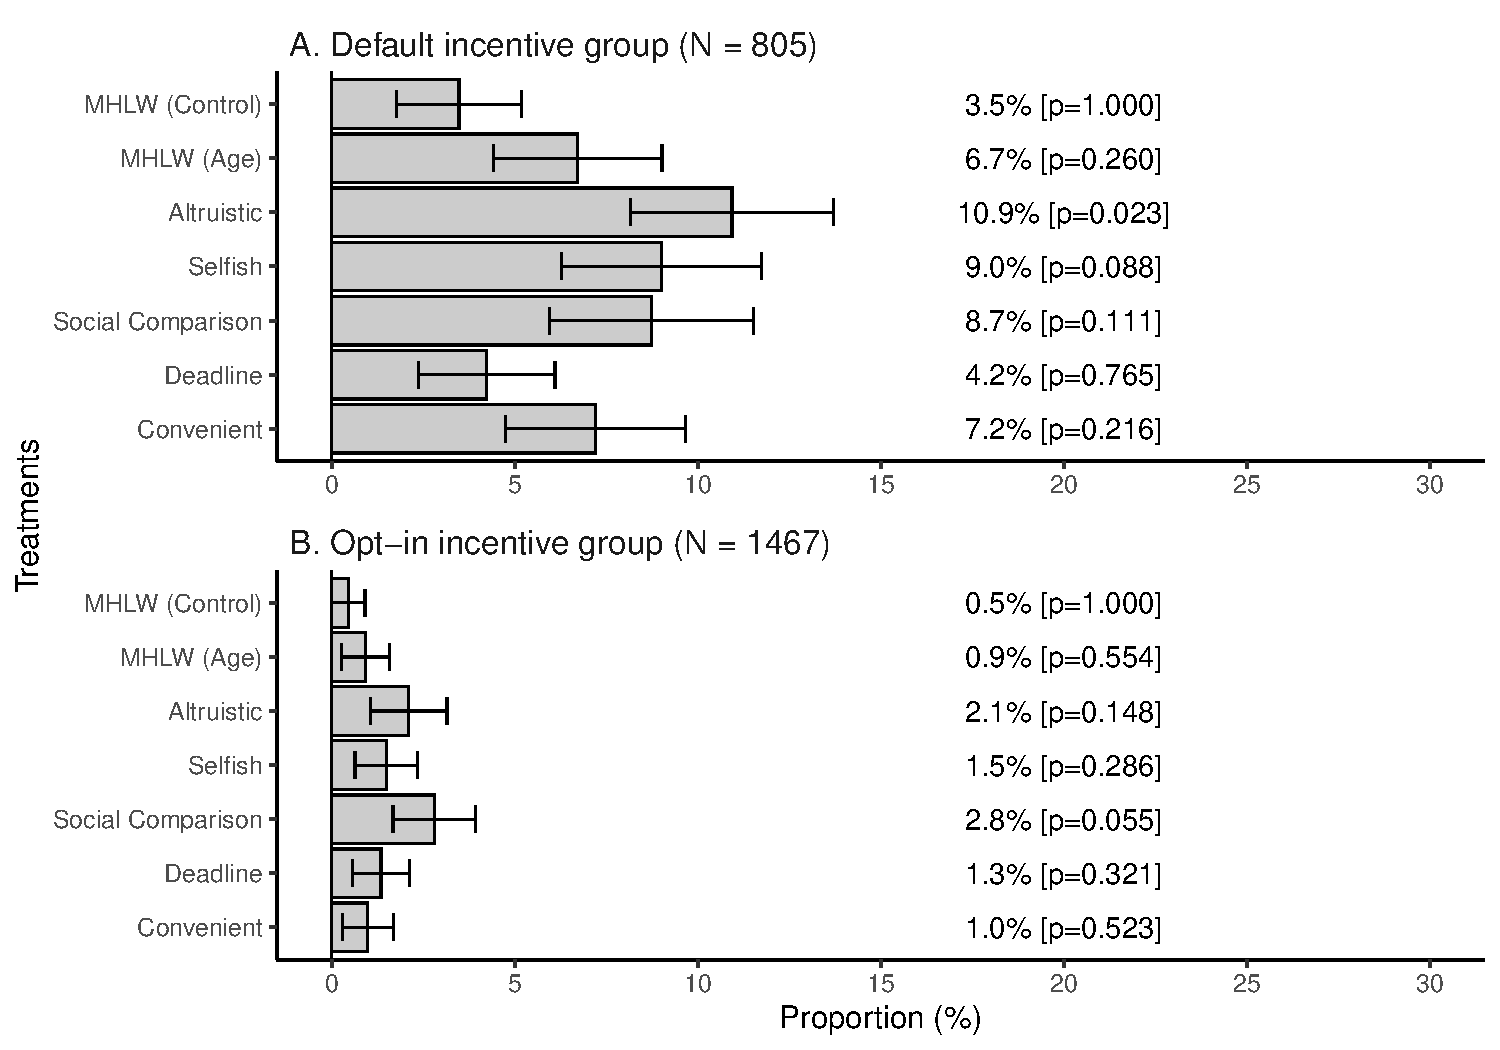
\includegraphics{Main-Document-LaTeX_files/figure-latex/ttest-act-test-1} \caption{Effect of the Text Message Reminders on the Actual Uptake of Antibody Testing. Notes: Numbers in the figure indicate the proportion of each experimental arm. Error bars indicate the standard error of the mean. Asterisks are p-values of t-tests for the difference-in-mean: * $p < 0.1$, ** $p < 0.05$, *** $p < 0.01$.}\label{fig:ttest-act-test}
\end{figure}

Figure \ref{fig:ttest-act-test} shows the actual uptake of antibody testing in each experimental arm for the \emph{default incentive} group (Panel A) and \emph{opt-in incentive} group (Panel B). As in the intention case, the Altruistic message statistically significantly increases the actual uptake of antibody testing compared with the MHLW (Control) message by \(7.4\) pp in the \emph{default incentive} group (\(10.9\)\% in the Altruistic message group versus \(3.5\)\% in the MHLW (Control) message group).

The Selfish message may boost the actual uptake of antibody testing in the \emph{default incentive} group by \(5.5\) pp (9\% in the Selfish message group versus \(3.5\)\% in the MHLW (Control) message group). Moreover, the Social Comparison message may also increase the actual uptake of antibody testing in the \emph{opt-in incentive} group (\(4.9\)\% in the Social Comparison message group versus \(3.5\)\% in the MHLW (Control) message group). These effects are statistically significant at the 10\% level.

\begin{figure}[t]
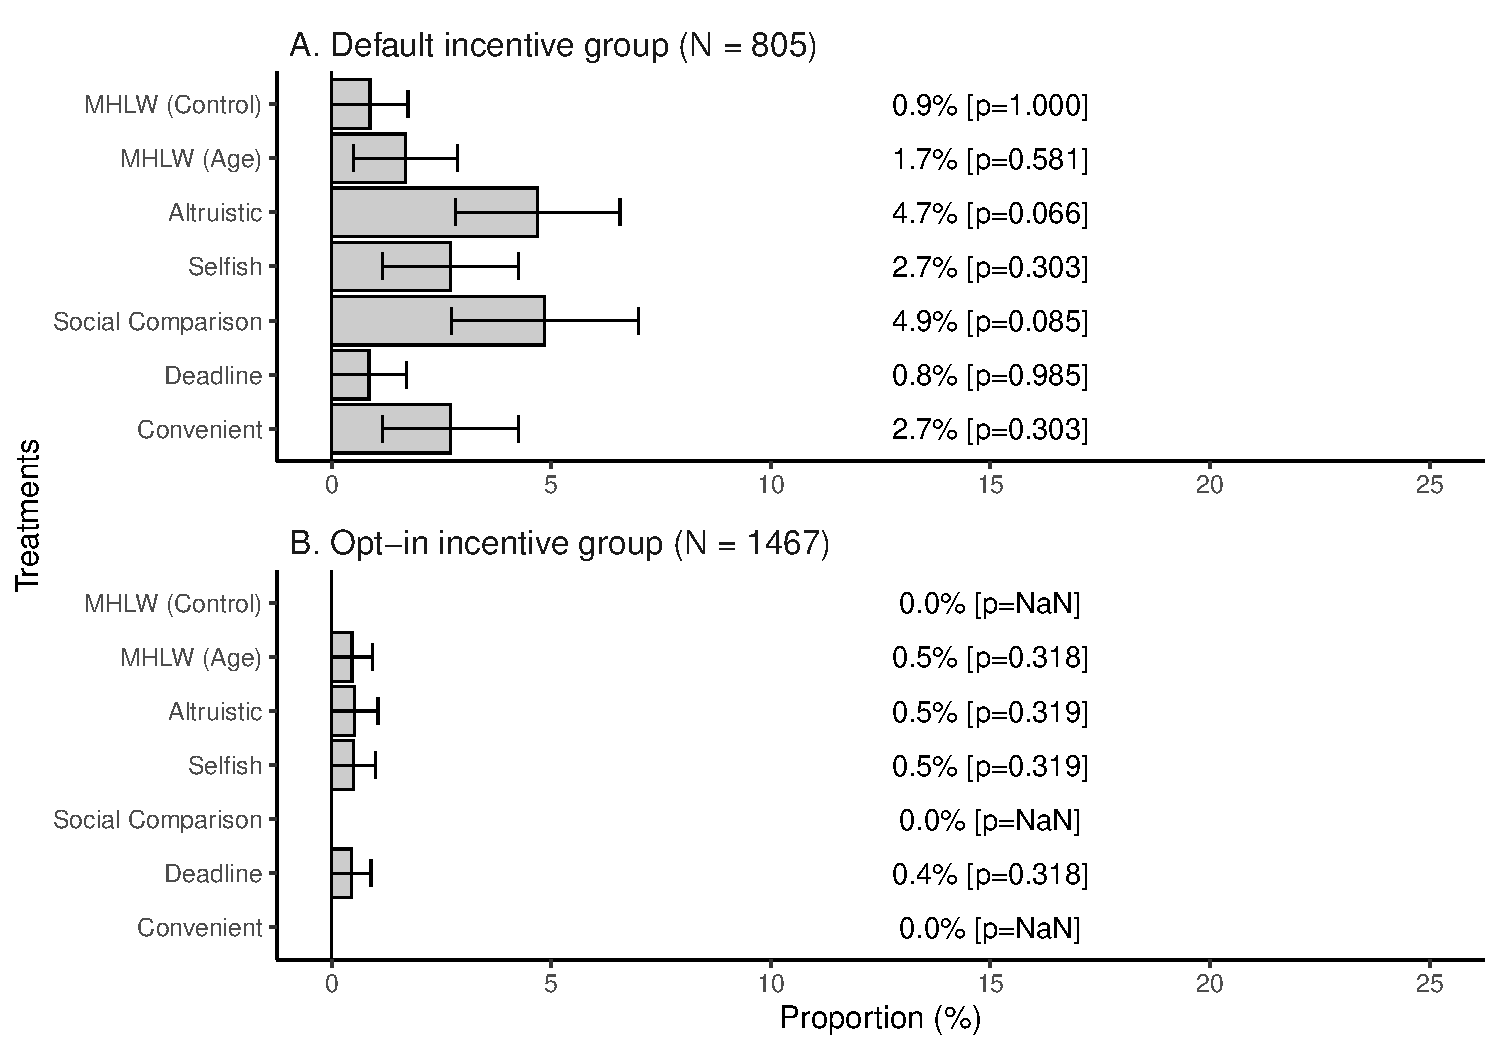
\includegraphics{Main-Document-LaTeX_files/figure-latex/ttest-act-vacc-1} \caption{Effect of the Text Message Reminders on Vaccination Rates. Notes: Numbers in the figure indicate the proportion of each experimental arm. Error bars indicate the standard error of the mean. Asterisks are p-values of t-tests for the difference-in-mean: * $p < 0.1$, ** $p < 0.05$, *** $p < 0.01$.}\label{fig:ttest-act-vacc}
\end{figure}

Figure \ref{fig:ttest-act-vacc} shows the vaccination rates in each experimental arm for the \emph{default incentive} group (Panel A) and \emph{opt-in incentive} group (Panel B).\footnote{Vaccination is a dummy variable coded 1 if the respondents were both tested and vaccinated. Thus, the vaccination rate can be regarded as the proportion of newly acquired antibodies through vaccination. This outcome variable matches the MHLW's policy goal.} In the \emph{default incentive} group, the Altruistic message may increase the vaccination rate by \(3.8\) pp (\(4.7\)\% in the Altruistic message group versus \(0.9\)\% in the MHLW (Control) message group). In the same group, the Social Comparison message may also increase vaccination rate by 4 pp (\(4.9\)\% in the Social Comparison message group versus \(0.9\)\% in the MHLW (Control) message group). These effects are statistically significant at the 10\% level.

\hypertarget{regression-analysis-1}{%
\subsubsection{Regression Analysis}\label{regression-analysis-1}}

\begin{table}

\caption{\label{tab:reg-act}Regressions of Behavior}
\centering
\fontsize{9}{11}\selectfont
\begin{threeparttable}
\begin{tabular}[t]{lcccc}
\toprule
\multicolumn{1}{c}{ } & \multicolumn{2}{c}{Testing} & \multicolumn{2}{c}{Vaccination} \\
\cmidrule(l{3pt}r{3pt}){2-3} \cmidrule(l{3pt}r{3pt}){4-5}
  & (1) & (2) & (3) & (4)\\
\midrule
MHLW (Age) & \num{0.032} & \num{0.028} & \num{0.008} & \num{0.005}\\
 & (\num{0.029}) & (\num{0.028}) & (\num{0.015}) & (\num{0.015})\\
Altruistic & \num{0.075}** & \num{0.072}** & \num{0.038}* & \num{0.037}*\\
 & (\num{0.033}) & (\num{0.032}) & (\num{0.021}) & (\num{0.020})\\
Selfish & \num{0.055}* & \num{0.060}* & \num{0.018} & \num{0.018}\\
 & (\num{0.032}) & (\num{0.032}) & (\num{0.018}) & (\num{0.017})\\
Social Comparison & \num{0.053} & \num{0.056}* & \num{0.040}* & \num{0.039}*\\
 & (\num{0.033}) & (\num{0.033}) & (\num{0.023}) & (\num{0.023})\\
Deadline & \num{0.008} & \num{0.005} & \num{0.000} & \num{-0.002}\\
 & (\num{0.025}) & (\num{0.025}) & (\num{0.012}) & (\num{0.012})\\
Convenient & \num{0.037} & \num{0.037} & \num{0.018} & \num{0.017}\\
 & (\num{0.030}) & (\num{0.030}) & (\num{0.018}) & (\num{0.018})\\
Opt-in & \num{-0.030}* & \num{-0.019} & \num{-0.009} & \num{-0.004}\\
 & (\num{0.018}) & (\num{0.020}) & (\num{0.009}) & (\num{0.012})\\
MHLW (Age) $\times$ Opt-in & \num{-0.028} & \num{-0.026} & \num{-0.003} & \num{-0.001}\\
 & (\num{0.030}) & (\num{0.030}) & (\num{0.015}) & (\num{0.016})\\
Altruistic $\times$ Opt-in & \num{-0.058}* & \num{-0.057}* & \num{-0.033} & \num{-0.032}\\
 & (\num{0.034}) & (\num{0.034}) & (\num{0.021}) & (\num{0.021})\\
Selfish $\times$ Opt-in & \num{-0.045} & \num{-0.054} & \num{-0.013} & \num{-0.013}\\
 & (\num{0.034}) & (\num{0.033}) & (\num{0.018}) & (\num{0.018})\\
Social Comparison $\times$ Opt-in & \num{-0.029} & \num{-0.034} & \num{-0.040}* & \num{-0.039}*\\
 & (\num{0.035}) & (\num{0.035}) & (\num{0.023}) & (\num{0.023})\\
Deadline $\times$ Opt-in & \num{0.001} & \num{0.004} & \num{0.005} & \num{0.007}\\
 & (\num{0.027}) & (\num{0.026}) & (\num{0.013}) & (\num{0.013})\\
Convenient $\times$ Opt-in & \num{-0.032} & \num{-0.031} & \num{-0.018} & \num{-0.018}\\
 & (\num{0.031}) & (\num{0.031}) & (\num{0.018}) & (\num{0.018})\\
\addlinespace[0.3em]
\multicolumn{5}{l}{\textbf{Linear combination test: Treatment + Opt-in $\times$ Treatment}}\\
\hspace{1em}MHLW (Age) (Opt-in incentive) & \num{0.005} & \num{0.003} & \num{0.005} & \num{0.004}\\
\hspace{1em} & (\num{0.008}) & (\num{0.009}) & (\num{0.005}) & (\num{0.005})\\
\hspace{1em}Altruistic (Opt-in incentive) & \num{0.017} & \num{0.016} & \num{0.005} & \num{0.005}\\
\hspace{1em} & (\num{0.011}) & (\num{0.011}) & (\num{0.005}) & (\num{0.005})\\
\hspace{1em}Selfish (Opt-in incentive) & \num{0.010} & \num{0.007} & \num{0.005} & \num{0.005}\\
\hspace{1em} & (\num{0.010}) & (\num{0.010}) & (\num{0.005}) & (\num{0.005})\\
\hspace{1em}Social Comparison (Opt-in incentive) & \num{0.023}* & \num{0.021}* & \num{0.000} & \num{0.000}\\
\hspace{1em} & (\num{0.012}) & (\num{0.013}) &  & (\num{0.001})\\
\hspace{1em}Deadline (Opt-in incentive) & \num{0.009} & \num{0.008} & \num{0.004} & \num{0.005}\\
\hspace{1em} & (\num{0.009}) & (\num{0.009}) & (\num{0.004}) & (\num{0.005})\\
\hspace{1em}Convenient (Opt-in incentive) & \num{0.005} & \num{0.007} & \num{0.000} & \num{0.000}\\
\hspace{1em} & (\num{0.008}) & (\num{0.009}) & (\num{0.000}) & (\num{0.001})\\
\midrule
Covariates &  & X &  & X\\
Num.Obs. & \num{2272} & \num{2272} & \num{2272} & \num{2272}\\
R2 & \num{0.030} & \num{0.047} & \num{0.019} & \num{0.029}\\
\bottomrule
\end{tabular}
\begin{tablenotes}
\item Notes: * $p < 0.1$; ** $p < 0.05$; *** $p < 0.01$. Robust standard errors are in parentheses. Covariates are age, years of education, annual income, usual health behavior (exercise, medical checkup, and annual influenza vaccination), and psychological factors potentially associated with the experimenter demand effect and social desirability bias (following social norms, accepting bad behavior in anonymous conditions). Effect of the text message reminders in the \emph{opt-in incentive} group is estimated by summing the main term of the treatment dummy and the cross-term between the treatment dummy and opt-in dummy.
\end{tablenotes}
\end{threeparttable}
\end{table}

As in the intention case, the different effects of the text message reminders for the two incentive groups are influenced by factors other than the presence or absence of free vouchers, including the age difference. Thus, we estimate the linear probability model \eqref{eq:regression}. Table \ref{tab:reg-act} shows the results.

The regression analysis also shows that the Altruistic message increases the actual uptake of antibody testing only in the \emph{default incentive} group. Controlling for the covariates, the Altruistic message increases the actual uptake of antibody testing by a statistically significant \(7.3\) pp in this group (column (2)). Furthermore, although the statistical significance is weak, the effect of this message falls by \(5.7\) pp as the cost of obtaining a free vaccination voucher increases. Hence, the effect of the Altruistic message in the \emph{opt-in incentive} group is \(1.6 (=7.3-5.7)\) pp, which is not statistically significant. The same trend is observed for the effect on vaccination rates, but statistical significance becomes weak.

As confirmed by the difference-in-means test, controlling for the covariates, the Selfish message increases the actual uptake of antibody testing in the \emph{default incentive} group, although the statistical significance is weak (column (2) in Table \ref{tab:reg-act}). In addition, the Social Comparison message may increases the actual uptake of antibody testing in both incentive groups, controlling for the covariates (column (2) in Table \ref{tab:reg-act}). However, the effect size is larger in the \emph{default incentive} group than in the \emph{opt-in incentive} group (not a statistically significant difference).

As confirmed by the difference-in-means test, the Social Comparison message may increase the vaccination rate in the \emph{default incentive} group (column (4) in Table \ref{tab:reg-act}). Although weakly statistically significant, the effect of this message lowers by \(5.7\) pp as the cost of obtaining vaccination vouchers increases. Hence, the Social Comparison message does not increase the vaccination rate in the \emph{opt-in incentive} group. Again, the effect of the Altruistic message follows a similar trend.

\hypertarget{influencing-mechanisms-of-the-altruistic-message}{%
\subsection{Influencing Mechanisms of the Altruistic Message}\label{influencing-mechanisms-of-the-altruistic-message}}

The text message reminders other than MHLW (Age) modify the age expression and message content. Thus, their effect relative to MHLW (Control) should be interpreted as the combined effect of the two modifications. Here, we examine which modification is more effective in the Altruistic message, which has a positive effect on both the intention to undertake antibody testing and the actual uptake of antibody testing in the \emph{default incentive} group. The only difference between the MHLW (Age) and MHLW (Control) messages is the age expression, while the only difference between the Altruistic and MHLW (Age) messages is the message content. Therefore, by estimating the effect of each difference, we can decompose the combined effect of the Altruistic message.

Compared with MHLW (Control), MHLW (Age) increases the intention to intention to undertake antibody testing in the \emph{default incentive} group by only \(2.1\) pp (\(22.9\)\% in the MHLW (Age) message group versus \(20.8\)\% in the MHLW (Control) message group; see Figure \ref{fig:ttest-int-test}), but this effect is not statistically significant. On the contrary, compared with MHLW (Age), the Altruistic message increases the intention to undertake antibody testing by \(12.2\) pp (\(35.1\)\% in the Altruistic message group versus \(22.9\)\% in the MHLW (Age) message group; see Figure \ref{fig:ttest-int-test}), which is statistically significant (Table 4 in Supplementary Material C).\footnote{Even in the \emph{opt-in incentive} group, the Altruistic message content may increase the intention to undertake antibody testing. Compared with the MHLW (Age) message group, the Altruistic message increases the intention to undertake antibody testing by \(7.7\) pp (\(32.9\)\% in the Altruistic message group versus \(25.2\)\% in the MHLW (Age) message group), which is statistically significant at the 10\% level. Moreover, only in the \emph{opt-in incentive} group does the content of the Convenient message statistically significantly increase the intention to undertake antibody testing by about 9 pp (Table 4 in Supplementary Material C). This group may lack an understanding of the routine immunization campaign. In fact, the Wave 1 survey shows that only about 20\% of the \emph{opt-in incentive} group were aware of the availability of routine vaccination.} Therefore, the effect of the Altruistic message on the intention to undertake antibody testing is strongly influenced by changing the message content.

Which individuals were influenced by the content of the Altruistic message? Since this message emphasizes the possibility that infected pregnant women may give birth to children with disabilities (CRS), we examine the differences in CRS knowledge and altruistic preferences. First, in Wave 1, we examine CRS knowledge and test the heterogeneity of the effect of the Altruistic message on the intention to undertake antibody testing depending on whether the respondents possessed such knowledge (see column (1) of Table 8 in Supplementary Material C). The results show that the Altruistic message content may be relatively more effective for those lacking such knowledge. Thus, the Altruistic message content may modify knowledge on the negative externalities of infection.

Second, we investigate whether the respondents feel pleasure in taking actions for others in Wave 1 and test the heterogeneous effects of the Altruistic message content (see column (2) of Table 8 in Supplementary Material C). The results show that the more altruistic a participant is, the stronger the effect of the Altruistic message content (this trend is statistically significant). Thus, the Altruistic message may be ineffective for those who do not care about others, even if they perceive negative externalities from reading messages.

Unlike in the intention case, the effect of the Altruistic message on the actual uptake of antibody testing is not solely due to the message content. Compared with MHLW (Age), which only changed the age expression, the Altruistic message increases the actual uptake of antibody testing by \(4.2\) pp (\(10.9\)\% in the Altruistic message group versus \(6.7\)\% in the MHLW (Age) message group). However, the regression analysis indicates that this increase is not statistically significant (Table 7 in Supplementary Material C). Further, modifying the age expression increases the actual uptake of antibody testing by \(3.2\) pp (\(6.7\)\% in the MHLW (Age) message group versus \(3.5\)\% in the MHLW (Control) message group), but not significantly. Thus, the effect of the Altruistic message on behavior is a combination of the addition of a simple age expression and revision of the message content.

\hypertarget{monetary-value-of-the-text-message-reminders}{%
\subsection{Monetary Value of the Text Message Reminders}\label{monetary-value-of-the-text-message-reminders}}

So far, we have examined the effects of combining financial incentives and nudges. The results show that the Altruistic message (and possibly the Social Comparison message) encourages men who received free vouchers by default (i.e., those who already received financial incentives) to undertake antibody testing and be vaccinated. Here, we evaluate the monetary value of adding nudges by examining how much more monetary compensation would be required if the effects of the combination were achieved by monetary compensation alone.

We first estimate the demand function using the WTP for the rubella vaccination.\footnote{Several studies calculate the monetary value of text message reminders. For example, \citet{Bursztyn2019} calculated it using the relative effects of financial incentives and text message treatment groups. \citet{Moriwaki2020} also surveyed WTP amounts and calculated monetary value. The latter study is similar to our approach.} We then examine the extent to which the corresponding cost (WTP) changes when the baseline vaccination rate is increased by the effect of the text message reminder. This cost change is the additional subsidy equivalent to the effect of the text message reminder. Since we want to estimate the monetary value of the text message reminder in the \emph{default incentive} group, the baseline vaccination rate is that when the vaccination cost is zero. Furthermore, since vaccination requires an exogenous condition that men do not have antibodies, we use the effect on the actual uptake of antibody testing. Since those willing to be vaccinated must undergo antibody testing, the effect on antibody testing should be viewed as the true intention to be vaccinated inferred from behavior. See Supplementary Material B for the detailed estimation method.

\begin{table}

\caption{\label{tab:monetary-value}Estimated Monetary Value of the Text Message Reminders}
\centering
\fontsize{9}{11}\selectfont
\begin{threeparttable}
\begin{tabular}[t]{lcccccc}
\toprule
\multicolumn{3}{c}{ } & \multicolumn{2}{c}{Monetary value (JPY)} & \multicolumn{2}{c}{Monetary value (USD)} \\
\cmidrule(l{3pt}r{3pt}){4-5} \cmidrule(l{3pt}r{3pt}){6-7}
Text message reminder & Effect & Baseline + effect & pp & total & pp & total\\
\midrule
MHLW (Age) & 0.032 & 0.732 & 367.854 & 1.946 & 3.679 & 17.690\\
Altruistic & 0.075 & 0.774 & 2037.553 & 10.779 & 20.376 & 97.988\\
Selfish & 0.055 & 0.755 & 744.045 & 3.936 & 7.440 & 35.782\\
Social Comparison & 0.053 & 0.752 & 596.335 & 3.155 & 5.963 & 28.678\\
Deadline & 0.008 & 0.707 & 86.059 & 0.455 & 0.861 & 4.139\\
Convenient & 0.037 & 0.737 & 422.789 & 2.237 & 4.228 & 20.332\\
\bottomrule
\end{tabular}
\begin{tablenotes}
\item We use the effect size of each text message reminder on the actual update of antibody testing. Baseline is the sum of the actual uptake of antibody testing in the control group and the vaccination rates under no vaccination cost estimated by the demand function. The monetary value is the amount per person multiplied by the number of people who received the voucher in 2019 but did not use it until January 2020 ($5.29$ million). USD 1 = JPY 110. The unit of monetary value per person is 1 JPY and 1 USD, respectively. The unit of total monetary value is 1 billion JPY and 1 million USD, respectively.
\end{tablenotes}
\end{threeparttable}
\end{table}

Table \ref{tab:monetary-value} shows the estimated monetary value of the text message reminders. The second and third columns show their effect on the actual uptake of antibody testing and the baseline vaccination rates plus the reminder effect, respectively. As shown in the fourth column, the Altruistic and Social Comparison messages, which promote antibody testing, have monetary values of about JPY 2,000 (about USD 18; 40\% of the assumed vaccination cost) and JPY 600 (USD \(5.5\); 12\%), respectively.\footnote{We elicit the WTP for the vaccination, assuming the vaccination costs JPY 5,000.} The total monetary value is the product of the per capita value and number of people who have not yet used the free vouchers issued in FY2019 (\(5.29\) million as of January 2020). As shown in the fifth column, the Altruistic and Social Comparison messages are worth JPY 10 billion (about USD 98 million) and JPY 3 billion (about USD 28 million), respectively.

\hypertarget{conclusion}{%
\section{Discussion and Conclusions}\label{conclusion}}

This study uses RCTs to investigate effective messages for promoting rubella antibody testing and vaccination in two situations using financial incentives. Our experiment reveals that the Altruistic message, which emphasizes the negative externality of infection, increases the intention to undertake antibody testing by \(14.3\) pp among men who received free vaccination vouchers in FY2019. This message is particularly effective for those unaware of the negative externalities of infection and for altruistic individuals who consider the benefits of others. Moreover, the Altruistic message also has a positive effect on the actual uptake of antibody testing. Among men who received vaccination vouchers in FY2019, the Altruistic message increases the actual uptake of antibody testing by \(7.5\) pp, which is equivalent to subsidizing 40\% of the vaccination cost.

However, the Altruistic message is less effective for men who incur transaction costs to obtain the vaccination vouchers. There may be a statistically significant difference in the effect of this message between the two groups. This finding suggests that text message reminders are effective when closely combined with financial incentives. In addition to the Altruistic message, the Selfish and Social Comparison messages raise the intention to undertake antibody testing and actual uptake of antibody testing among men who already received the vaccination vouchers by default. However, these effect sizes are insufficiently large to maintain statistical power, thereby requiring re-examination with a larger sample size.

One potential concern in this study is that all the behavior-related outcomes were self-reported and may contain recall bias; however, these biases are less problematic because Wave 2 measures behavior within the last month. The self-reported behavioral outcomes may also be subject to the experimenter demand effect and social desirability bias. To address these biases, our regression analysis directly controls for the respondents' psychological factors potentially associated with these biases (e.g., following social norms, accepting bad behavior in anonymous conditions). Even if these biases cannot be eliminated, they are not fatal to identifying the effect of the text message reminders since this study is an RCT and these biases exist to the same extent in each group.

Finally, we offer two directions for future research. First, why are text message reminders ineffective in groups that must incur transaction costs to obtain the free vaccination vouchers? Our messages may not increase the value of antibody testing and vaccination sufficiently to outweigh their cost. Another possibility is the low awareness of the rubella immunization campaign (approximately 77.5\% of the respondents were unaware of the campaign). Thus, even if they read the messages and realized the importance of antibody testing and vaccination, they would have believed they had to pay for these preventive actions.\footnote{The fact that many people are unaware of the additional routine rubella vaccination precludes the possibility that they stopped getting antibody testing and were vaccinated in the first year (FY2019) because they expected to automatically receive the voucher the following year.}

The second direction concerns the channels of the effect on vaccination rates. We find that the Altruistic and Social Comparison messages may increase vaccination rates among men who received free vaccination vouchers by default. The effect of the text message reminders on vaccination rates is created through two channels. First, the messages increase the number of negative individuals who need to be vaccinated. Second, the messages encourage unvaccinated negative individuals to be vaccinated. Our data suggest that the first channel is more important than the second. Table 9 in the Supplementary Material C shows the number of men who underwent antibody testing, who had a negative antibody test, and who were vaccinated in each experimental arm in the \emph{default incentive} group. Most of those with negative antibody test results were vaccinated in all the experimental arms. Furthermore, the number of negative antibody tests varied between the experimental arms. In particular, 25\% of the antibody tests were negative in the MHLW (Control) message group compared with 50\% (\(=7/14\)) and 56\% (\(=5/9\)) for the Altruistic and Social Comparison messages, respectively, which may have a positive effect on vaccination rates.\footnote{The negative rate of antibody testing for the Selfish message, which is only effective for the actual uptake of antibody testing, was 30\% (\(=3/10\)). This value is similar to that for the MHLW (Control) message.} Thus, the experimental arms with higher vaccination rates have a greater negative antibody testing rate, resulting in a positive effect on vaccination.

This argument is related to targeting interventions \citep[e.g.,][]{Finkelstein2019}. The question is whether marginal individuals whose behavior is changed by an intervention receive significant benefits from a policy. In our context, the Altruistic message increases the number of individuals receiving negative antibody test results , who receive a large benefit from the FY2019 vaccination campaign. Thus, the Altruistic message improves targeting. However, since we cannot test the difference in the rates of negative antibody tests because of our small sample, this remains a topic for future research.

\clearpage

\bibliography{text-message-2020RCT.bib}



\end{document}
